\chapter{Generic Chapter}
This is a generic chapter of your thesis. Remember to put ANY chapter in a different source file (including introduction and all the others). 

For the purpose of this guide, the main \LaTeX constructs and how to use them will be explained here. Other thematic chapters will follow, i.e., which will trace the chapters that should be present in your thesis. Delete this generic chapter once you have learned this contents.

You can write in italic \emph{like this}, you can write in bold \textbf{like this}, or you can write using colors \textcolor{cyan}{like this}.

This is an \emph{itemize}, where you can put a list of items, like this:
\begin{itemize}
\item item number 1
\item item number 2
\end{itemize} 

This is an \emph{enumerate}, where you can put a list of items with numbers, like this:
\begin{enumerate}
\item item number 1
\item item number 2
\end{enumerate} 

You can cite references like this: \cite{lee2016introduction} \cite{jiang2013towards}, by using the \lstinline{\cite} directive. You have to copy within \lstinline{\cite} brackets the label of the entry that you have in the BibTeX file (\texttt{.bib}). The \texttt{.bib} file of this thesis is \texttt{mybib.bib}. he command \lstinline{\addbibresource} at the top of this main file indicates what BibTeX file you are referring to. 

As an example, this is a BibTeX entry:

\begin{verbatim}
@inproceedings{urias2018cyber,
  title={Cyber Range Infrastructure Limitations and Needs of Tomorrow: A Position Paper},
  author={Urias, Vincent E and Stout, William MS and Van Leeuwen, Brian and Lin, Han},
  booktitle={2018 International Carnahan Conference on Security Technology (ICCST)},
  pages={1--5},
  year={2018},
  organization={IEEE}
}
\end{verbatim}

For every online paper that you may read on online libraries, you can download its BibTeX entry. For example:
\begin{enumerate}
	\item For IEEE Xplore, click on the paper name, then click on ``Cite This'', ``BibTeX'', and you can find the entry;
	\item For Google Scholar, click on the ``Cite'' voice under the paper name, then click ``BibTeX'', and you can find the entry. 
\end{enumerate}

Just copy and paste such an entry in the .bib file. If you find a paper on Scholar that is nevertheless published by IEEE, by convention you should take the entry from the IEEE website and not from Scholar. To do this, just click on the title of the paper. This will redirect you to the resource page on IEEE Xplore. Once here, follow instructions at point 1.

When you compile, a correct number will automatically be assigned to the citation in the text, and the complete entry will appear at the bottom of the document, in the ``Bibliography'' chapter. 

If you need to cite a generic online resource, which does not necessarily correspond to a scientific paper, use the \lstinline{@misc} entry in the \texttt{.bib} file. A \lstinline{@misc} entry looks like this:

\begin{verbatim}
@misc{nist2018,
    author = "{NIST}",
    title = "Cyber Ranges",
    year = "2018",
    howpublished = "\url{https://www.nist.gov/system/files/documents/2018/02/13/cyber_ranges.pdf}",
    note = "[Online; Accessed 2019, 28 November]"
  }
\end{verbatim}

You have to manually create this entry from scratch and manually type these fields. Remember not to forget any of these fields. You can choose the label with which to refer to the resource. The title of the website (which you can see at the top of the tab of your browser showing the page) can be used as the title of the resource.

In general, enter a citation of this type for sites only when there are data, phrases, or images that you intend to report. Instead, if you want to cite names of software or hardware devices, prefer the use of the \lstinline{\footnote}, in which you will only have to specify the URL of the item. 

Remember that citations, both in the text and in the image captions, usually go to the end of a sentence, before the fullstop, as in this case \cite{vykopal2017kypo}. In case of long periods, they can also be placed before other detachment signs, such as commas or semicolons, or colons if they precede a list, itemized or enumerated. An exemption is allowed in the event that the name of research projects, described in some scientific resource, is being introduced, as in this case:

\begin{center}
Cybertropolis \cite{deckard2018cybertropolis} is described in a very good paper by Gary Deckard.
\end{center}

Remember to put citations very often to justify your claims, especially when you report data or results. Just consider them as a justification of what you, in an original way, are writing. Citations are not needed to have permission to copy and paste sentences from online resources, which should NEVER be done - always try to rephrase the concept with your words.

\begin{figure}[h!]
\vspace{0.5cm}
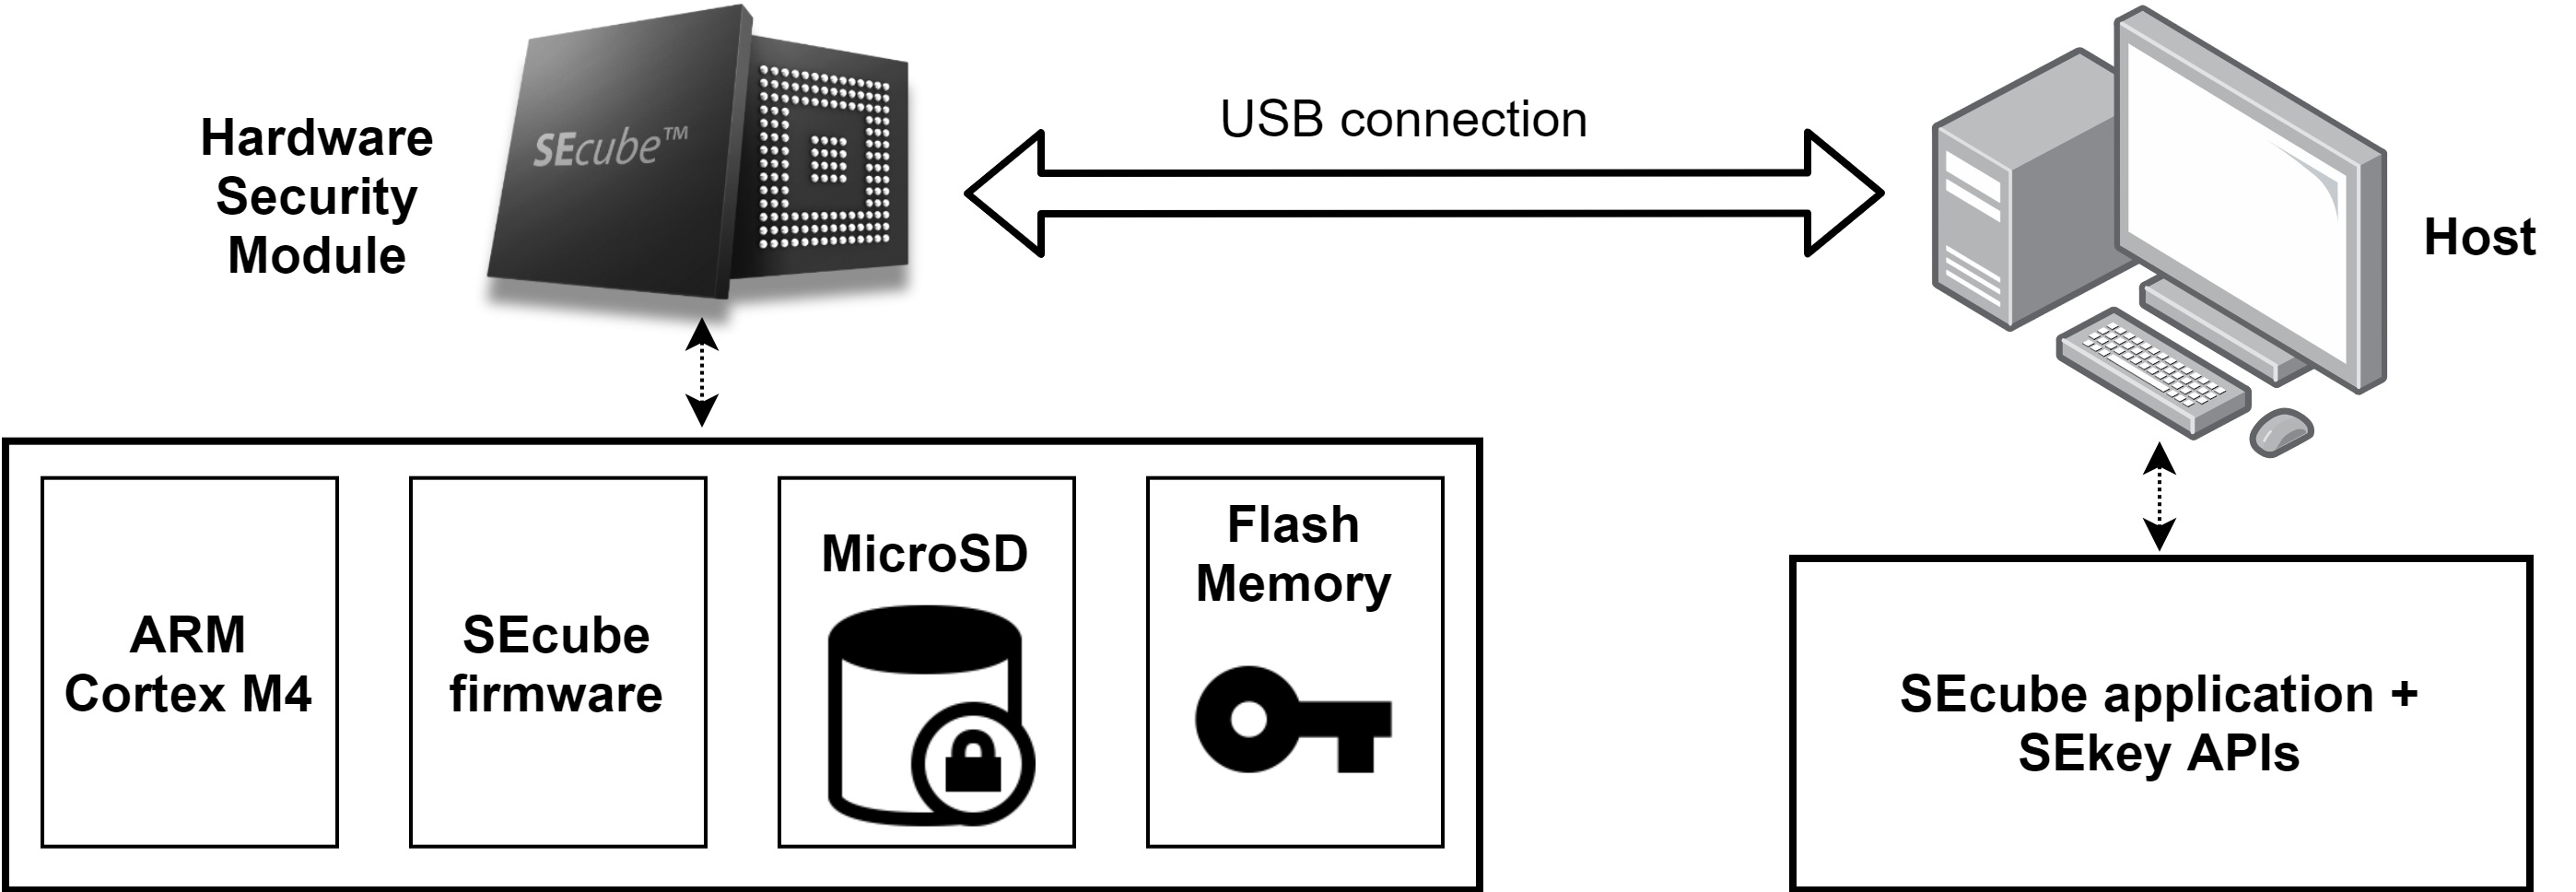
\includegraphics[width=\textwidth]{images/simplearch.jpg}
\caption{This is the image \emph{caption}.}
\label{fig:generalschema} % This is the image label, with which you can refer to the image in any document location.
\end{figure}

This is an image example. Images must ALWAYS be understandable: never introduce images that have text smaller than the text in your document. If you create the images yourself, try not to make them clash too much with the style of your document, and use the same font as this thesis.
If they are not images of your own creation, you MUST reference them. In the caption of the image, you need to insert a citation to the resource from which you took the image, at the end of the caption sentence, before the fullstop.
Each image you enter MUST be referenced in the text, using a formula similar to this:

\begin{center}
Figure \ref{fig:generalschema} describes the architecture of the system.
\end{center}

You can refer to the image using \lstinline{\ref} followed by the image label, that you put in the \lstinline{\label} entry of the figure. Remember to use the word Figure with a capital F. 

Remember that the more your text is adorned with figures, the more understandable, appreciable and readable it becomes.

\section{Section title}\label{examplesection}
This is a section under a chapter. The number of sections also contributes to greater readability of your text, and to a better display of the content in the index. In fact, sections are automatically shown in the Table of Contents. However, try not to make sections shorter than two pages. For smaller portions of your text, use subsections.

You can refer to a section using its label, using the \lstinline{\ref} directive as for images, like this:

\begin{center}
This concept has been explained in Section \ref{examplesection}.
\end{center}

Remember to use the word Section with a capital S. This is also valid for chapters. 

\subsection{Subsection title}
This is a subsection under the section. 

The following is a table.

\begin{table}
\centering
\caption{Preliminary Experimental Results}
\begin{tabular}{| p{3cm} | p{3cm} | p{3cm} |}
    \hline
    \textbf{Benchmark} & \textbf{Inputs} & \textbf{Processing time} \\ \hline
    SHA & Message of 100 KB & 368449 s \\ \hline
    RIJNDAEL & Message of 100 KB & 1083568 s \\ \hline
    DIJKSTRA & Matrix of 100x100 32-bit integers & 324782 s \\ \hline
    STRING & 1331 50-char strings & 178616 s \\ \hline
    BITCOUNT & 12800 32-bit integers & 419545 s \\ \hline
    \hline
\end{tabular}
\label{tab:ar}
\end{table}

If you want to write a formula, you can do like this:

\begin{equation}\label{eq:thiseq}
X_{k}=\sum _{n=0}^{N-1}x_{n}e^{-ik{\frac {2\pi }{N}}n}\quad \quad k=0,\dots ,N-1
\end{equation}

Tables and formulas are extensively documented online, and any doubts about their syntax can be easily resolved with a simple search. As for figures and sections, the same rules also apply to tables and formulas: mandatory reference in the text, possibility to use \lstinline{\label} to label them, and naming with capital letter (e.g., ``as in Table \ref{tab:ar}, as in Formula \ref{eq:thiseq}).

The following is a piece of code:

\begin{lstlisting}
int func(int N, int M) {
  float (*p)[N][M] = malloc(sizeof *p);
  if (!p)
    return -1;
  for (int i = 0; i < N; i++)
    for (int j = 0; j < M; j++)
      (*p)[i][j] = i + j;
  print_array(N, M, p);
  free(p);
  return 1;
}
\end{lstlisting}

You can customize the style of your code, changing the language, the colors of keywords, of comments or the background by changing the settings inside the \lstinline{\lstset} directive found in the main file. Usually, the listings are not referenced within the text as happens for figures, tables, formulas and sections. Do not overdo the code within your text: use it only for short passages (e.g., function prototypes, or 2 to 5 lines of code within a function to help the reader in better understanding the meaning of the text).

You can also write in-text code using the \lstinline{\lstinline} directive, \\
like this: \lstinline{int main(int argc, char** argv);}.

